%%% template.annotated.tex
%%%
%%% This LaTeX source document can be used as the basis for your technical
%%% paper or abstract. Unlike ``template.tex,'' this version of the source
%%% document contains documentation of each of the commands and definitions
%%% that should be used in the preparation of your formatted document.
%%% 
%%% The parameter given to the ``acmsiggraph'' LaTeX class in the 
%%% ``\documentclass'' command controls several features of the formatted 
%%% output: the presence or absence of hyperlinked icons just prior to the 
%%% first section of the paper, the amount of space left clear for the ACM
%%% copyright notice, the presence or absence of line numbers and submission
%%% ID, and the presence or absence of an appropriate ``preprint'' notice.
%%% 
%%% If you are preparing a paper for presentation in the Technical Papers
%%% program at one of our two annual flagship conferences, held in North 
%%% America (SIGGRAPH) or Asia (SIGGRAPH Asia), you should use ``annual''
%%% as the parameter.
%%%
%%% If you are preparing a paper for presentation at one of our sponsored
%%% events, including SIGGRAPH and SIGGRAPH Asia, but not in those events' 
%%% Technical Papers program, you should use ``sponsored'' as the parameter.
%%% (Technical Briefs and Game Papers presented at our annual flagship 
%%% events fall into this category, as do papers accepted to other SIGGRAPH-
%%% sponsored events, such as I3D or ETRA or VRCAI.)
%%%
%%% If you are preparing a version of your content for review, you should
%%% use ``review'' as the parameter. Line numbers will be added to your 
%%% paper, and the submission ID value will be printed across the top of 
%%% each page of your paper. (Use the submission ID as the parameter to the
%%% ``TOGonlineID'' command, below.)
%%%
%%% If you are preparing an abstract, typically one to four pages in 
%%% length, you should use ``abstract'' as the parameter. No space will 
%%% be left clear for the ACM copyright notice, as copyright is not 
%%% transferred for abstracts. A small permission notice will be added
%%% to your content during production in the footer of the first page.
%%%
%%% If you are preparing a preprint of your content, you should use
%%% ``preprint'' as the parameter. This is primarily for annual conference
%%% papers; a header reading ``To appear in ACM TOG X(Y)'' will appear on
%%% each page of the formatted output (where X is the volume and Y is the 
%%% number of the issue in which it will be published).

\documentclass[review]{acmsiggraph}

\usepackage{algpseudocode}
\usepackage{algorithm}



\newcommand{\npar}{\par \vspace{2.3ex plus 0.3ex minus 0.3ex} \noindent}
\newcommand{\spar}{\par \noindent}
\newcommand{\todo}[1]{\textcolor{red}{\(\langle\) \textbf{TODO} #1 \(\rangle\) }}

%%% Definitions and commands that begin with ``\TOG'' are meant to be used
%%% in the preparation of papers to be presented in the Technical Papers
%%% program at one of our annual flagship events - SIGGRAPH and SIGGRAPH 
%%% Asia. You can safely ignore these definitions and commands if your 
%%% content is to be presented in some other venue.

%%% ``\TOGonlineid'' should be filled with the online ID value you received
%%% when you submitted your technical paper. It will be printed out if you 
%%% prepare a ``review'' version of your paper.

\TOGonlineid{--}

%%% Should your technical paper be accepted, you will be given three pieces
%%% of information: the volume and number of the issue of the ACM Transactions
%%% on Graphics journal in which your paper will be published, and the 
%%% ``article DOI'' value, which is unique to your paper and provides the 
%%% link to your paper's page in the ACM Digital Library. Fill in the 
%%% ``\TOGvolume,'' ``\TOGnumber,'' and ``\TOGarticleDOI'' definitions with
%%% the three pieces of information you receive.

\TOGvolume{0}
\TOGnumber{0}
\TOGarticleDOI{1111111.2222222}

%%% By default, your technical paper will contain hyperlinked icons which 
%%% point to your paper's article page in the ACM Digital Library, and to 
%%% the paper itself in the ACM Digital Library. You may wish to add one 
%%% or more links to your own resources. If any of the following four 
%%% definitions have URLs in them, an appropriate hyperlinked icon will be
%%% added to the list. 

\TOGprojectURL{}
\TOGvideoURL{}
\TOGdataURL{}
\TOGcodeURL{}

%%% Define the title of your paper here. Use capital letters as appropriate.
%%% Setting the entire title in upper-case letters is not correct, nor is 
%%% capitalizing only the first letter of the title.

\title{The Title of Your Paper Goes Here}

%%% Define the author list in the ``\author'' command. The ``\thanks'' 
%%% field can be used to define an e-mail address for the author.
%%% The ``\pdfauthor'' field should contain a comma-separated list of the
%%% authors of the paper, and is used, along with the title and keyword
%%% data, for PDF metadata. (To see this metadata, open the PDF in Adobe 
%%% Reader and select ``File > Properties > Description.''

\author{Robert A. Smith\thanks{e-mail:rsmith@gmail.com}\\Smith Research}
\pdfauthor{Robert A. Smith}

%%% User-defined keywords.

\keywords{monte carlo rendering, filter, distribution effects, global illumination}

%%% End of the document preamble, start of the document.

\begin{document}

%%% A ``teaser'' image appears below the title and affiliation and above
%%% the two-column body of the paper. This is optional, but if you wish
%%% to include such an image, the commented-out code, below, can be used
%%% as an example. Please note that the inclusion of a ``teaser'' image
%%% may move the copyright space to the bottom of the right-hand column
%%% on the first page of your formatted output. This is acceptable.

%% \teaser{
%%   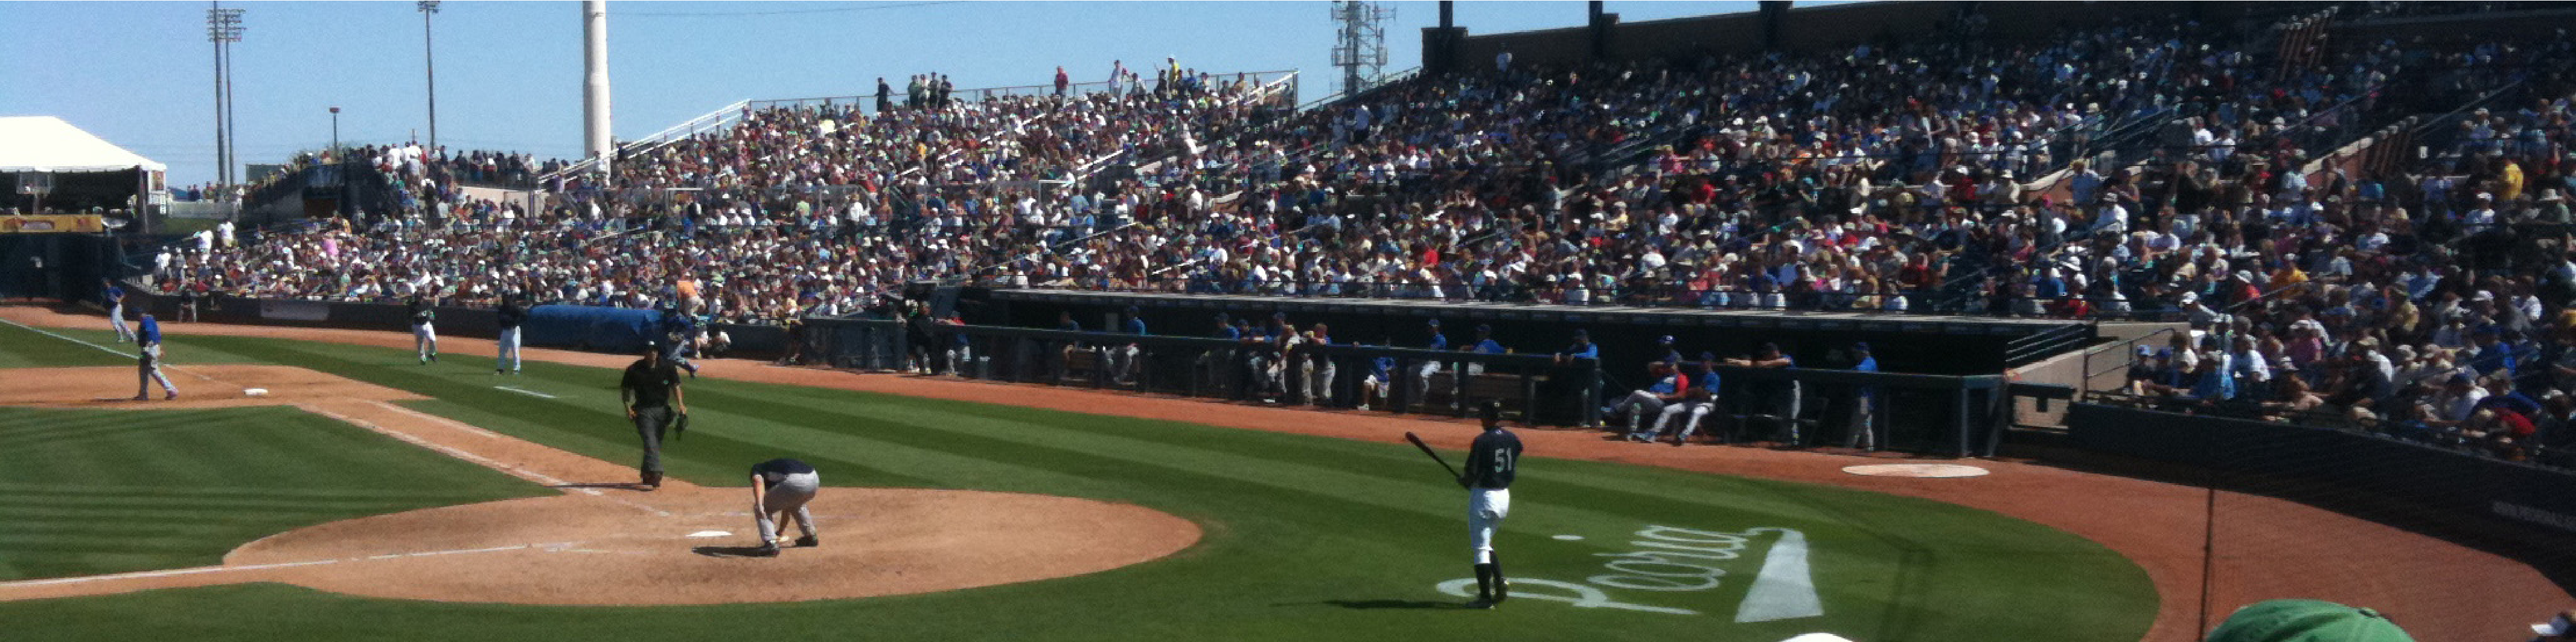
\includegraphics[height=1.5in]{images/sampleteaser}
%%   \caption{Spring Training 2009, Peoria, AZ.}
%% }

%%% The ``\maketitle'' command uses the author and title information 
%%% defined above, and prepares the formatted title.

\maketitle
\todo{pick title}

%%% The ``abstract'' environment should contain the abstract for your
%%% content -- one to several paragraphs which describe the work.

\begin{abstract}

When rendering using Monte Carlo methods, either a large amount of samples are necessary or noise will be present in the image.
A lot of methods have already tried to tackle this problem including adaptive sampling, reconstruction techniques and advanced image filtering techniques.
In this paper I will recapitulate the work I have done for my thesis so far. 
The focus will be on the RPF algorithm called random parameter filtering (RPF) as proposed in ~\cite{RPF11}.
As this algorithm is based on a cross bilateral filter, this concept will be explained and discussed as well.
To conclude, some other methods that handle the noise caused by Monte Carlo rendering at low sampling rates were investigated as well.
\todo{verwijs naar meerdere methodes die dit hebben proberen aan te pakken?}~\cite{dutré2006advanced}

%Citations can be done this way~\cite{Jobs95} or this more concise 
%way~\shortcite{Jobs95}, depending upon the application.

%Ut wisi enim ad minim veniam, quis nostrud exerci tation ullamcorper
%suscipit lobortis nisl ut aliquip ex ea commodo consequat. Duis autem
%vel eum iriure dolor in hendrerit~\cite{Pellacini:2005:LAH}
%in vulputate velit esse molestie~\cite{notes2002} 
%consequat, vel illum dolore eu feugiat nulla facilisis at vero eros et
%accumsan et iusto odio dignissim qui blandit praesent luptatum zzril
%delenit augue duis dolore te feugait nulla facilisi.~\cite{Park:2006:DSI}


\end{abstract}

%%% The ``CRCatlist'' environment defines one or more ACM ``Computing Review''
%%% (or ``CR'') categories, used for indexing your work. For more information
%%% on CR categories, please see http://www.acm.org/class/1998.

\begin{CRcatlist}
  \CRcat{I.3.7}{Computer Graphics}{Three-Dimensional Graphics and Realism}{Raytracing};
\end{CRcatlist}
\todo{CRcatlist}

%%% The ``\keywordlist'' prints out the user-defined keywords.

\keywordlist

%%% If you are preparing a paper to be presented in the Technical Papers
%%% program at one of our annual flagship events (and, therefore, using 
%%% the ``annual'' parameter to the ``\documentclass'' command), the 
%%% ``\TOGlinkslist'' command prints out the list of hyperlinked icons.
%%% If you are using any other parameter to the ``\documentclass'' command
%%% this command does absolutely nothing.

\TOGlinkslist

%%% The ``\copyrightspace'' command will leave clear an amount of space
%%% at the bottom of the left-hand column on the first page of your paper,
%%% according to the parameter used in the ``\documentclass'' command.

\copyrightspace

%%% The first section of your paper. 

\section{Introduction}
Computer Graphics has evolved from 2D to almost realistic 3D during the last decennia.
To reach this realism in graphics, Global Illumination algorithms became very important, 
these incorporate the indirect light caused by the surroundings.
These algorithms require large numbers of calculations and thus a large rendering time, especially when results without noise are expected.
To lower this rendering time, Monte Carlo methods are often used because they can be used to evaluate multidimensional functions in an unbiased way.
Complex and photorealistic images can be created using these Monte Carlo methods.
In the case of (Monte Carlo) rendering, the multidimensional integrals that needs to be solved at every pixel of the image are: 
integration of the radiance over the aperture of the camera (u,v), over the time the shutter is open ($t_0 \rightarrow t_1$) and over the area of the pixel ($(i-1/2,j-1/2) \rightarrow (i+1/2,j+1/2)$. 

\[
  I(i,j) = \int\limits_{i-\frac{1}{2}}^{i+\frac{1}{2}} 
		\int\limits_{j-\frac{1}{2}}^{j+\frac{1}{2}} 
		      \cdots
			  \int\limits_{-1}^{1} 
			      \int\limits_{-1}^{1}
				  \int\limits_{t_0}^{t_1} 
				    f(x,y,\cdots,u,v,t)
				  \,dt
			      \,dv
			  \,du
		\,dy
	    \,dx.
\]

As Monte Carlo methods take random samples to evaluate a function, a lot of samples are usually necessary to evaluate the function precisely and 
thus a lot of noise will be present when using a low number of samples. 
One obvious solution to this problem is to use more samples, 
but as the rendering time increases dramatically with the amount of samples this is not always an option.
Adaptive sampling algorithms can then be used to distribute these (sometimes large) numbers of samples in the best possible way across the image.
Reconstruction techniques can also be used to suppress the number of samples, 
as these try to use the available samples as much as possible, across pixels and even across frames.
Another technique that can be used is the focus of this paper and is an advanced image filter, 
it uses not only the color computed at each sample of the image, 
but also other parameters that are available during the rendering process, to filter the image.
\\
In the related work section I will describe all the different related papers I researched before deciding to research the RPF algorithm in more detail.
The technical sections describe the concept of bilateral filter after which the RPF algorithm is explained in detail.
To conclude the results describe my current results followed by a discussion of these results and a concise conclusion.


\section{Related Work}
\todo{plak de verschillende paper uitleggen aan elkaar, sorteer volgens jaar ???}
More information about Monte Carlo methods can be found here~\cite{kalos2009monte}, 
while more information about advanced rendering can be found here~\cite{dutré2006advanced} and here \cite{pharr2010physically}.
Some recent work that try to tackle the problem of noise at low sampling rates when using Monte Carlo rendering are discussed below.

%\todo{2010: integration  Compressive estimation for signal integration in rendering} \\
\textbf{Compressive estimation for signal integration in rendering:} \\ 
While Monte Carlo methods are used to evaluate functions, 
other methods like the one explained in ~\cite{Sen:CompressiveSignalEstimation:2010} can also be used to compute the integral of an unknown function.
This is possible because of the theory of compressed sensing, which allows to reconstruct a signal from a few linear samples if it is sparse in a transform domain.
This method can also be used to compute computer graphics distribution effects like anti-aliasing and motion blur.
The advantage of this function over Monte Carlo methods is that is needs only a few samples to estimate the function.
\\

%\todo{Temporal Light Field Reconstruction for Rendering Distribution Effects}
\textbf{Temporal Light Field Reconstruction for Rendering Distribution Effects:} \\
A general reconstruction technique that tries to maximize the image quality based on a given set of samples is given in ~\cite{Lehtinen2011sg}.
This technique exploits the dependencies in the temporal light field and allows efficient reuse of samples between different pixels.
The effective sampling rate is multiplied by a large factor when using this technique.
The paper makes the following four contributions:
\begin{enumerate}
  \item \textit{\textbf{The reconstruction algorithm}} \\
    The input of the algorithm contains a set of samples in the form:
    \begin{equation}
      s = \{(x,y,u,v,t) \rightarrow (z,v,L)\}
    \end{equation}
    With xy the screen coordinates, uv the lens coordinates, t the time, z the depth, v the 3D motion vector and L the radiance associated with the input sample.
    \\
    The reconstruction algorithm then goes as follows:
    \begin{enumerate}
     \item The screen coordinates of the input samples are reprojected to the (u,v,t) coordinates of the reconstruction location.
      Samples that are too far away from the reconstruction location in xy are discarded.
     \item The returned clusters of samples are grouped into apparent surfaces.
     \item If multiple apparent surfaces are found, they are sorted front-to-back.
      Afterwards, it is determined which one covers the reconstruction location.
     \item The output color is computed by filtering the samples that belong to the covering surface using a circular tent filter.
    \end{enumerate}

    
  \item \textit{\textbf{Determining visibility consistency}} \\
    By using the key observation that the relative ordering of the sreen positions of samples from a non-overlapping surface never changes under reprojections, 
    they derive a formal criterion named SAMESURFACE to detect when a set of reprojected samples should be filtered together.
  \item \textit{\textbf{Resolve visibility without explicit surface reconstruction}} \\
    Which surface is visible at the reconstruction location is determined. 
    The challenge is to distinguish between small holes in the geometry and apparent holes caused by stochastic sampling. 
    To do this a radius R is precomputed, R is the radius of the largest empty circle that is expected to be visible on the xy plane after reprojection. 
    Holes that are smaller than R should be filled because it is beyond the resolution of the input sampling. 
    The visibility is then determined using the following rule. 
    A reconstruction location is covered if it is possible to find three reprojected input samples that form a triangle that covers the reconstruction location and fits inside a circle of radius R.
  \item \textit{\textbf{Hierarchical query structure}} \\
    The reconstruction algorithm needs to retrieve the input samples that reproject to the vicinity of reconstruction location’s (x, y), given (u, v, t) quickly.
    The input samples are organized into a bounding volume hierarchy, where the extents of the nodes xy are parameterized using u, v and t. 
    When executing a query, the parameterized bounding volume is used to test if the reconstruction location is inside the bounds.
\end{enumerate}

%\todo{Reconstruction the Indirect Light Field for Global Illumination}
\textbf{Reconstruction the Indirect Light Field for Global Illumination:} \\
The algorithm that is described in ~\cite{Lehtinen:2012:RIL:2185520.2185547} is similar to the former algorithm and is published by almost the same authors.
The paper also describes a general reconstruction technique that exploits anisotropu in the light field and permits efficient reuse of input samples between pixels or world-space locations, 
multiplying the effective sampling rate by a large factor.
\\
The main difference between the two algorithms is that this algorithm tries to reconstruct the indirect light field at scene point instead of at points on the lens like the algorithm in ~\cite{Lehtinen2011sg} does.
That is also why reconstructing an image using this algorithm takes three to four times longer than the former algorithm. 
The former algorithm uses a 2D hierarchy, but this algorithm needs to reconstruct the incident light field at arbitrary points in the scene, so a true 3D algorithm is needed.
\\

%\todo{2012: adaptive filtering -- Axis-Aligned Filtering for Interactive Sampled Soft Shadows}
\textbf{Axis-Aligned Filtering for Interactive Sampled Soft Shadows:} \\
The post-processing step needed in Light Field Reconstruction techniques is very expensive.
Other algorithms like the one proposed in ~\cite{UdayMehta:2012:AAF} has a very simple filtering step by using axis-aligned filters.
Because of this extremely simple step, this algorithm can be integrated in real-time raytracers.
Adaptive filtering is used because the parameters of the used filters are adjusted depending on the input samples.
This algorithm is basically an image filter for noise that is fixed on the soft shadows effect.
\\

%\todo{2012: adaptive sampling -- Adaptive Rendering with Non-Local Means Filtering}
\textbf{Adaptive Rendering with Non-Local Means Filtering:} \\
The following algorithm found in ~\cite{Rousselle:2012:ARN:2366145.2366214} describes an adaptive sampling algorithm for Monte Carlo rendering.
An adaptive sampling algorithm tries to determine the optimal sample distribution across the image.
This can be done by allocating more samples to regions with difficult light effects.
The first step of the algorithm distributes a given budget of samples over the image after which the image is filtered in the second step of the algorithm with a variant of the NL-means filter which is a generalisation of the bilateral filter.
This filter considers distances between pairs of pixel values to compute filter weights, the term non-local is caused by the fact that the set of samples that contribute to one output pixel can come from a large region in the input image.
In the third step of the algorithm the remaining error in the filtered image is estimated to drive the adaptive sampling in the next iteration step.
\\

%\todo{2008: adaptive sampling -- Multidimensional Adaptive Sampling and Reconstruction for Ray Tracing}
\textbf{Multidimensional Adaptive Sampling and Reconstruction for Ray Tracing:} \\
A combination of adaptive sampling and reconstruction is proposed in ~\cite{Hachisuka:2008:MAS:1360612.1360632}.
This paper introduces a new sampling strategy for ray tracing.
The samples on which the strategy operates are generated from the rendering equation directly and are thus not generated through Monte Carlo sampling.
Additionally this algorithm uses all previously generated samples to generate a new sample.
After sampling this high-dimensional function, a reconstruction is made by integrating the function over all but the image dimensions.
\\

%\todo{2012: adaptive sampling reconstruction  SURE-based Optimization for Adaptive Sampling and Reconstruction}
\textbf{SURE-based Optimization for Adaptive Sampling and Reconstruction:} \\
A similar goal is aimed for by ~\cite{Li:2012:SBO} allthough samples are distributed over the image based on an estimator of the Mean Squared Error (MSE) of the image.
The estimator that is used is called Stein's Unbiased Risk Estimator (SURE), it allows to estimate the error of an estimator without knowing the true value that is estimated.
Another difference is that a filterbank is used instead of a single filter.
The usage of a filterbank makes this algorithm different from algorithms like RPF because any kind of filter can be added to this filterbank.
The authors of the paper have experimented with isotropic Gaussian, cross bilateral and a modified non-local means filter.
A small number of initial samples are rendered first, followed by filtering each pixel with all filters in the filterbank.
Next the filtered color with the lowest SURE error is chosen for each pixel and is used in the reconstruction.
When more samples are available, these are used for the pixels with the largest SURE errors after which the process goes back to filtering each pixel with all the filters from the filterbank.
\\

%\todo{2011: adaptive sampling reconstruction  Adaptive sampling and reconstruction using greedy error minimization}
\textbf{Adaptive sampling and reconstruction using greedy error minimization:} \\
Another algorithm that does not fix which filter is used for different pixels is described in ~\cite{Rousselle:2011:ASR:2070781.2024193}.
As this algorithm is greedy, it minimizes the function at each stage hoping to reach a global optimum.
Given a current sample distribution, a filter that minimizes the pixel error is selected from a discrete set of filters that can be different for each pixel.
Given the filter selection, addition samples are distributed to further reduce the MSE.
Because the MSE cannot be calculated exactly the change in MSE is calculated instead.
This whole process can be repeated until any chosen termination criterion is met.
\\

%\todo{2011: Visibility  High-Quality Spatio-Temporal Rendering using Semi-Analytical Visibility}
\textbf{High-Quality Spatio-Temporal Rendering using Semi-Analytical Visibility:} \\
A visibility technique with the only purpose to render motion blur with per-pixel anti-aliasing is described in ~\cite{Gribel2011}.
A number of line samples are used over a rectangular group of pixels that form a 2D spatio-temporal visibility problem together with the time dimension.
This problem needs to be solved per line sample.
Each group of pixels in the image is rendered separately.
For each group a Bounding Volume Hierarchy is used to receive only the geometry that overlaps with the tile. 
Furthermore each line sample is processed one at a time by calculating what triangles intersect with the sample followed by resolving the depth visibility.
When all the triangles have been processed, the final visibility is resolved and for each pixel the contribution of the line samples overlapping the pixel is accumulated to the color of that pixel.
\\

%\todo{2012: visibility sampling  A Theory of Monte Carlo Visibility Sampling}
\textbf{A Theory of Monte Carlo Visibility Sampling:} \\
~\cite{Ramamoorthi:2012:ATO} tries to lower the amount of noise introduced by Monte Carlo sampling of the visibility term in the rendering equation.
By analysing the effectiveness of different non-adaptive Monte Carlo sampling patterns for rendering soft shadows, 
they search for the pattern with the lowest expected variance for a certain visibility function.
These results can lead to a reduction in the needed number of shadow samples without losing precision by using the best sampling pattern.
\\

\section{Bilateral Filter}
The Bilateral filter is introduced in ~\cite{710815}, I have used some extra information from ~\cite{bilfilter} as well.
\\
As the name already suggests, a bilateral filter filters an image using two different inputs.
To understand the working of a bilateral filter, the concept of a Gaussian filter is explained first.

\subsection{Gaussian filter}
As an image has two dimensions, the 2D version of the gaussian filter will be explained, in fact this is simply the product of two one dimensional gaussians, one per direction.
The equation of a 2D Gaussian filter is defined as:

\begin{equation}
   g(x,y) = \frac{1}{2\pi\sigma^2}e^{-\frac{x^{2}+y^{2}}{2\sigma^{2}}}
\end{equation}

with x and y being the distance from the origin and $\sigma$ being the standard deviation of the Gaussian distribution.
The shape of a Gaussian filter being a 2D bell shaped function.
\\
When an image is filtered using a Gaussian filter, this will lead to blurred images as the values of each pixel will fade into the values of the surrounding pixels.
\todo{Add a Gaussian filtered image!!}

\subsection{Bilateral filter as two Gaussian filters}
A bilateral filter can be explained as being two Gaussian filter that filter respectively in the spatial (the domain filter D) and in the intensity domain (the range filter R).

\begin{equation}
  \begin{aligned}
    D(x,y) &=& e^{-\frac{x^{2}+y^{2}}{2\sigma^{2}}} \\
    R(p_i, p_j) &=& e^{-\frac{f(p_i)^{2}+f(p_j)^{2}}{2\sigma^{2}}}
  \end{aligned}
\end{equation}

The domain filter filters using the difference x and y between the positions of the two pixels and the range filter uses the intensity value (obtained by the image function $f$) of both pixels.
\\
We can now write down the equation to compute final value of a pixel filtered using a bilateral filter.

\begin{equation}
\begin{aligned}
   b(p_i) &=& k^{-1}\sum_{m=0}^{N-1} f(p_m)D(x,y)R(p_i,p_m) \\
   \text{with} \\
   k &=& \sum_{m=0}^{N-1} D(x,y)R(p_i,p_m)
\end{aligned}
\end{equation}

x and y are again the difference in the positions of the pixels $p_i$ and $p_m$ and N is the size of the neighboorhood taken into account for each pixel.


\subsection{Cross Bilateral Filter}
The RPF algorithm that is described in the following section, is based on a more advanced version of a bilateral filter, called the cross bilateral filter.
A Cross bilateral filter does not only filter in the spatial and the intensity domain but adds another filtering function to the filter.
This added function is a function just like the image function and returns a value for each position in the image.
Examples of this function are the world position at the first intersection point of the ray traced through that pixel, other features like the normal can also be chosen.


\section{Random Parameter Filtering algorithm}

\todo{Mutual information}
\todo{different parts of algorithm}
\\
\subsection{General information}
The algorithm Random parameter filtering introduced in ~\cite{RPF11} tries to reduce the noise caused by the random parameters used in Monte Carlo integration.
This noise reduces when the sampling rate increases, but this also increases the rendering time which is often not desirable.
A Monte Carlo renderin system calculates the colors of the pixels using a function like this:
\[
 c_i \Leftarrow f(p_{i,1},p_{i,2};r_{i,1},r_{i,2},\cdots,r_{i,n})
\]

with f being the function of the scene with inputs $p_i$ being the position of the sample and the random parameters $r_i$.
As the RPF algorithm is a post-process filter and uses a lot more than only the colors of the samples to filter the image, the following data has to be collected by the rendering system and given to the RPF algorithm as input:
\[
 x_i = \{p_{i,1},p_{i,2};r_{i,1},\cdots,r_{i,n};f_{i,1},\cdots,f_{i,m};c_{i,1},c_{i,2},c_{i,3}\}
\]

For each sample a vector like this is stored, containing the position of the sample $p_i$, the random parameters $r_i$ needed to compute the sample colors $c_i$ and the scene features $f_i$.
These scene features are the extra features on which the cross bilateral filter also filters, in particular the features that are used are
the world-space position, normal and texture values for the first intersection point of the ray and the world position and normal for the second intersection when using path tracing.
When a feature is not available for a certain sample it is replaced with a zero.

The algorithm itself computes the statistical dependency between the outputs and the inputs of the rendering system.
This information is then used in the filter to adjust the importance of the sample value.
\\
An example can clarify this process, an image that is rendered using depth of field:
regions that are in focus are free of noise because a ray that goes through the lens from a focused point on the image will land on the same point in the scene, regardless of where on the lens the random point is located.
For pixels out of focus on the other hand, the color of the sample depends on the random lens position.

\subsection{Implementation of the algorithm}
A detailed description on how the RPF algorithm is implemented can be found in ~\cite{RPFTechReport}.
The algorithm consists of three big parts which will be explained seperately.

\begin{algorithm}
  \caption{RPF algorithm}
  \label{algo:RPF}
  \begin{algorithmic}
    \State filterSize[] = ${55,35,17,7}$
    \For  {$t=0$ to $filterSize.length$} 
      \For {all pixels P in image I} 
	 \State Preprocess samples in neighboorhood N of P based on 
	 \State filterSize[t]
	 \State Compute statistical dependencies of sample color and 
	 \State features on inputs $p_i$ and $r_i$, use them to compute filter 
	 \State weights.
	 \State Filter sample colors in P using the weighted cross 
	 \State bilateral filter.
      \EndFor
    \EndFor \\
    Box filter all samples of each pixel to compute the final pixel color \\
    \Return filtered image
  \end{algorithmic}
\end{algorithm}

\subsubsection{Multiple iterations}
While a filter with a neighboorhood size of the entire image would be desirable, this is not feasible because of the computation overload 
(to filter one sample all the samples in the neighboorhood have to be used).
To solve this problem multiple iterations with different neighboorhood sizes are used.
By experimenting, the authors found four iterations with the following sizes to be sufficient: ${55,35,17,7}$.
By going from a large to a small size, the low frequency noise is filtered first followed by filtering more and more detail noise.

\subsubsection{Preprocess samples in Neighboorhood N of P based on the filtersize}
In this part of the algorithm a vector of samples is created to use in the computation of the filter weights.
Because the number of samples increases as $O(N^2)$ with the block size, a smaller number of random samples are chosen from within the neighboorhood.
These samples are then clustered, this means that the random sample is only added to the neighboorhood if all of its scene features are within three standard deviations of the mean for the pixel.
This test is only done when the standard deviation of that scene feature for the pixel is bigger than 0.1, this makes sure that not all samples are thrown away when the variance is very small.
\\
Before the statistical dependencies are computed for this newly created neighboorhood, all the elements in the sample vector are normalized by removing the mean and deviding by the standard deviation of all samples in the neighboorhood.
This makes sure that all features get an equal weight when calculating dependencies.

\subsubsection{Compute statistical dependencies and the filter weights}
First Mutual information is explained as this technique is used to calculate the statistical dependencies between a sample feature and the inputs to the Monte Carlo system.
\\

\textbf{Mutual Information}
The technique of mutual information is described in ~\cite{cover2006elements} as a measure of the amount of information that one random variable contains about another random variable.
The mutual information of two random variables X and Y with a joint probability mass function $p(x,y)$ and marginal probability mass function $p(x)$ and $p(y)$ is given by:

\[
 I(X,Y) = \sum_{x\in X} \sum_{y\in Y} p(x,y)log\frac{p(x,y)}{p(x)p(y)}
\]

To implement the computation of the mutual information between two vectors, the histogram of each of them as well as their joint histogram is computed.
The marginal histograms are computed by making all the values positive first by subtracting the minimum element and quantize the elements to integers.
Then the number of times a value occurs is then counted after which these values are devided by the length of the vector.
The joint histogram is implemented very similarly like in ~\cite{jointhistogram} using the positive and quantized vectors.
The number of times each couple of values occurs is calculated using a 2D array after which each element is divided by the length of the vectors.

\textbf{Computing the filter weights}
Two vectors with filter weights are needed, $\alpha$ and $\beta$.
$\alpha$ is the vector containing the weights used for the color term, one value for each color channel.
$\beta$ contains the weights used for the feature term, one value for each scene feature.
After the computation of the dependencies of the colors of the samples with the random parameters, the positions and the scene features, the filter weights that are used for the color values can be computed with the following equations:

\begin{equation}
 \begin{aligned}
 \alpha_k &=& max(1-2(1+0.1t)W_{c,k}^{r},0) \\
 \beta_k &=& W_{c}^{f,k}max(1-(1+0.1t)W_{f,k}^{r}, 0)
 \end{aligned}
\end{equation}

with $W_{c,k}^r$ the fractional contribution of the random parameters on the $k^{th}$ color channel,
$t$ the number of the block size, $W_{f,k}^{r}$ the fractional contribution of the random parameters on the $k^{th}$ scene feature and
$W_{c}^{f,k}$ the fractional contribution of the $k^{th}$ scene feature  on the color.
The normalized dependency on the random parameters gets more weight as the block size goes down with each iteration.

\subsubsection{Filter the samples using the weighted cross bilateral filter}
After the computation of the filter weights, the filtering of the samples is done simply using algorithm~\ref{algo:filter}

\begin{algorithm} 
  \caption{Filter the samples}
  \label{algo:filter}
  \begin{algorithmic}
    \For  {all samples i in P} 
      \State $c_i^{''} \leftarrow 0, w \leftarrow 0$
      \For {all samples j in N} 
	 \State Calculate $w_{ij}$ with equation~\ref{eq:weight}
	 \State $c_i^{''} \leftarrow c_i^{''} + w_{ij}c_i^{'}$
	 \State $w \leftarrow w + w_{ij}$
      \EndFor
      \State $c_i^{''} \leftarrow \frac{c_i^{''}}{w}$
    \EndFor \\
    \Return filtered color of the samples $c^{''}$
  \end{algorithmic}
\end{algorithm}

\begin{equation} \label{eq:weight}
  \begin{aligned}
 w_{ij} = &exp&(-\frac{1}{2\sigma_{c}^{2}}\sum_{1\leq k\leq3}\alpha_k(c_{i,k}-c_{j,k})^2)* \\
	  &exp&(-\frac{1}{2\sigma_{f}^{2}}\sum_{1\leq k\leq m}\beta_k(f_{i,k}-f_{j,k})^2)
  \end{aligned}
\end{equation}

Because the samples in the neighboorhood are selected using a Gaussian distribution the position term of the bilateral filter could be dropped.
The variances of the filter are:

\begin{equation}
 \begin{aligned}
    \sigma_c^{2} = \sigma_f^{2} &=& \frac{\sigma^2}{(1-W_c^r)^2} \\
    \text{with } \\
    \sigma^2 &=& 8\sigma_8^2/s
 \end{aligned}
\end{equation}

with $s$ the samples per pixel and $\sigma_8^2$ the experimentally selected variance of $0.02$ for noisy scenes or $0.002$ for all others.



\section{Results}
\todo{vergeet niet PBRT2 te vermelden}
\section{Discussion}
\todo{stel resultaten voor en beschrijf en interpreteer ze, welke zijn de sterke-zwakke punten, welke problemen zijn nog niet helemaal opgelost, eventueel vergelijkingen met gelijkaardige systemen, enz.}
\\

\section{Conclusion}
\todo{typische een zeer korte summary + conclusie van je werk}

Lorem ipsum dolor sit amet, consectetur adipisicing elit, sed do
eiusmod tempor incididunt ut labore et dolore magna aliqua. Ut enim ad
minim veniam, quis nostrud exercitation ullamco laboris nisi ut
aliquip ex ea commodo consequat. Duis aute irure dolor in
reprehenderit in voluptate velit esse cillum dolore eu fugiat nulla
pariatur. Excepteur sint occaecat cupidatat non proident, sunt in
culpa qui officia deserunt mollit anim id est laborum.

\section*{Acknowledgements}
\todo{KULEUVEn en de makers van RPF enzo..}

%To Robert, for all the bagels.

%%% Please use the ``acmsiggraph'' BibTeX style to properly format your
%%% bibliography.

%%% Please use the ``acmsiggraph'' BibTeX style to properly format your
%%% bibliography.

\bibliographystyle{acmsiggraph}
\bibliography{nieuwepaper}
\end{document}